\newpage
\section{Theorie}
\label{sec:theorie}

\subsection{Bestimmung des Schubmoduls $G$}
Um das Schubmodul $G$ zu bestimmen wird ein zylindrischer Stab oder Draht des zu untersuchendes
Materials in eine Vorrichtung gespannt. Bei dieser ist das obere Ende fest fixiert und das untere
Ende kann gedreht werden, so dass auf das Material eine Schubspannung wirkt.

\begin{figure}[h]
    \centering
    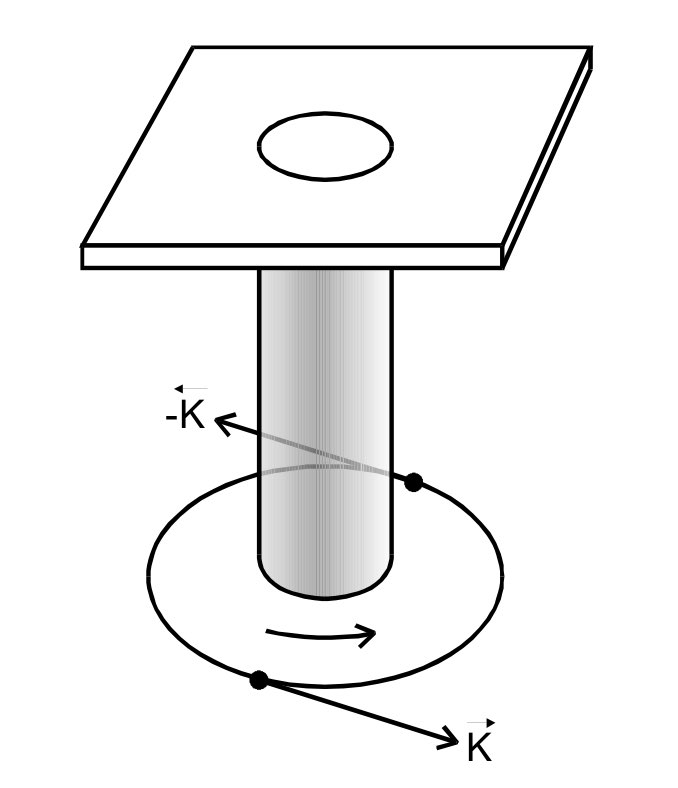
\includegraphics[width=0.35\textwidth, height=0.4\textwidth]{bilder/Torsion_allgemein.jpeg}
    \caption{Torsion eines Drahtes/Stabes,\cite[5]{Anleitung}}        
    \label{fig:torsion_allgemein}
\end{figure} 

Die zwei entgegengesetzen Kräfte $K$ wirken dabei auf zwei gegenüberliegenden Punkten 
und führen zu einer Deformation des Körpers.

Mit der Beziehung  %\eqnref{eqn:def_schubmodul} 
und dem Scherungswinkel $\alpha$, Torsionwinkel $\phi$ 
und der Körperlange $L$ folgt:
\begin{equation}
    M = \int_{0}^{R} 2\pi\;\frac{G}{L}\;\phi r^3 dr = \frac{\pi}{2}G\frac{R^4}{L}\phi
\end{equation}
Mit der Richtgröße $D$
\begin{equation}
    D:=\frac{\pi G R^4}{2L}
    \label{eqn:richtgroesse}
\end{equation}

Hierbei spielt die elastische Nachwirkung aus \ref{sec:nachwirken_vorb} eine bedeutenden Rolle.
Um diese Fehlerquelle zu minimieren, nutzt man statt dieser (in Abbildung \ref{fig:torsion_allgemein} dargestellten) 
Statischen Methode eine Dynmaische
Methode an, bei der die Schubspannung zeitlich periodische wirkt und zusätzlich eine Kugelmasse $m_\text{k}$ 
an den Draht befestigt wird.
Konkret wird diese Dynamische Methode später in Abschnitt \ref{sec:Durchfuehrung} erleutert.\\
\newpage
Somit führt eine Auslenkung aus der Gleichgewichtslage zu einer ungedämpften harmonischen
Drehschwingung mit der Periodendauer $T$ aufgrund der entgegenwirkenden Drehmomente $M_\text{Draht}$ 
und $M_\text{Masse}$:
\begin{equation}
    M_\text{Draht} + M_\text{Masse} = 0
\end{equation}
\begin{align}
    T & = 2\pi \sqrt{\frac{\theta}{D}} & \mathrm{mit} & &  \theta_\text{Kugel} = \frac{2MR^2}{5}
    \label{eqn:trägheitsmoment}
\end{align}
wobei $\theta$ das Trägheitsmoment einer Kugel ist.\\

Mit Gleichung \ref{eqn:richtgroesse} und \ref{eqn:trägheitsmoment} folgt somit:
\begin{equation}
    G=\frac{16 \pi m_\text{k}R^2_\text{k}L}{5T^2R^4}
    \label{eqn:schubmodul_formel}
\end{equation}


\subsection{Das magnetische Moment eines Permanentmagneten}
Für das magnetische Moment $\vec{m}$ gilt
\begin{equation}
    \vec{m_\text{mag}}:=p\;\vec{a}
\end{equation}
mit $p$ als Polstärke und $\vec{a}$ als Abstand zwischen den Polen.\\
Befindet sich der Magnet in einem homogene B-Feld, resultiert ein Magnetisches Drehmoment.
\begin{equation}
    M_\text{Mag} = m\;B\;sin(\gamma)
\end{equation}

\begin{figure}[h]
    \centering
    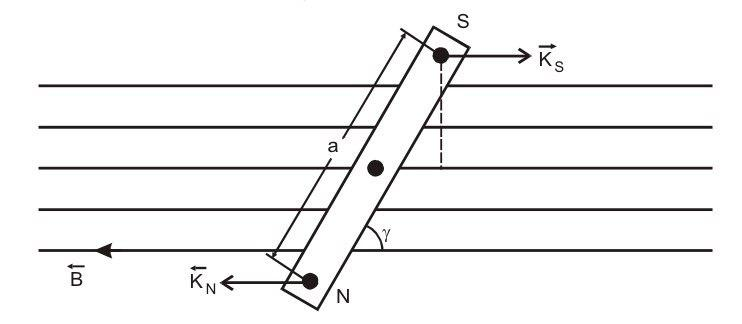
\includegraphics[width=0.35\textwidth, height=0.15\textwidth]{bilder/Drehmoment.jpg}
    \caption{Permanentmagneten in einem äußeren Magnetfeld $\vec{B}$,\cite[12]{Anleitung}}        
    \label{fig:drehmoment}
\end{figure}

Mit einer Kleinwinkelnäherung ergibt sich für die Periodendauer $T_\text{m}$:
\begin{equation}
    T_\text{m} = 2\pi\;\sqrt{\frac{\theta}{mB\;+\;D}}\\
    \label{eqn:periode}
\end{equation}

